\classheader{2018-06-15}

Compare the following:
\begin{equation*}
	\circled{a} \quad \frac{dy}{dx} = x - e^{x/2} \quad \quad
	\circled{b} \quad \frac{dp}{dy} = \dfrac{p}{2} - 450
\end{equation*}

\begin{enumerate}[label=\protect\circled{\arabic*}]
	\item Both are First Order ODEs.
	\item Both are linear.
	\item \circled{a} us if the form $y' = f(x)$ and is simply a calculus problem (think finding $\int f(x) dx$)\\ Here the RHS is only a function of the independent variable
	\begin{itemize}
		\item Integrate both sides with respect to x to set $y(x) = \frac{x^2}{2} - 2e^{x/2} + c$
		\item This formula is called a \underline{general solution} to \circled{a} as it is an expression that specifies \underline{all} possible solutions.
		\item A \underline{particular solution} to \circled{a} involves choosing a value for the constant $'c'$
		\item Graphs of solutions are called \underline{integral curves}. The red line is when $c = 4$\\
		\begin{center}
		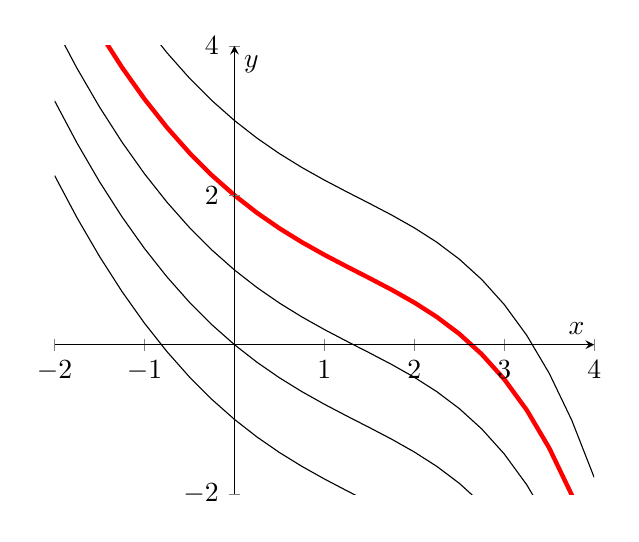
\begin{tikzpicture}
			\begin{axis}[
			xmin =-2, xmax=4,
			ymin=-2, ymax =4,
			axis lines=center,
			axis on top=true,
			domain=-2:4,
			xlabel={$x$},
    		ylabel={$y$},]
						
			\addplot[mark=none, draw=black, thin]{((x^2)/2) - (2*exp(x/2)) + 1};
			\addplot[mark=none, draw=black, thin]{(x^2/2) - 2*exp(x/2) + 2};
			\addplot[mark=none, draw=black, thin]{((x^2)/2) - (2*exp(x/2)) + 3};
			\addplot[mark=none, draw=red, ultra thick]{((x^2)/2) - (2*exp(x/2)) + 4};
			\addplot[mark=none, draw=black, thin]{((x^2)/2) - (2*exp(x/2)) + 5};
		
			\end{axis}

		\end{tikzpicture}
		\end{center}
	\item We also call the general solution to \circled{a} as \underline{1-parameter family of solutions}
	\end{itemize}
	With the addition of a single pt in the xy-plane (ex. $y(0) = 2$), called an \underline{initial value}, we can "choose" a particular solution from the family.\\
	With this point, there is now only 1 solution to the problem:
	\begin{equation*}
		y(x) = \frac{x^2}{2} - 2e^{x/2} + c
	\end{equation*}
	\begin{equation*}
		y(0) = \frac{x^2}{2} - 2e^{x/2} + c = 2
		= 0 -2 + c=2\Rightarrow \circled{c = 4}
	\end{equation*}
	Here the solution to the Initial Value Problem \textbf{(IVP)} (an ODE with initial values)
	\begin{center}
		$\underbrace{y' = x-e^{x/2}, \quad y(0)=2}_{\textbf{IVP}}$ is $y(x) = \frac{x^2}{2} - 2e^{x/2} + 4$
	\end{center}
	\item \circled{b} is not of the form $y' = f(x)$. Rather it is of the form $y' = f(y)$, where dependent variable on RHS.\\
	\underline{Note:} This is harder to solve but easier to study!
	\begin{definition-N}
		if in an ODE the independent variable is \underline{NOT} explicitly present, the ODE is called \underline{autonomous}.
	\end{definition-N}
	\redhline\\
	Let's solve \circled{b}: there are many ways. We choose something like what we will eventually call "separation of variables"\newline \\
	First recall from Calculus I:
	\begin{enumerate}[label=\protect\circled{\Roman*}]
	\item For any diff. $p(t)$, the function $p(t)$ and $p(t) - 900$ have the same derivative: $p'(t)$
	\item $\dfrac{d}{dt}[ln|f(t)] = \dfrac{f'(t)}{f(t)}$ for $f(t)$ differentiable and $f(t) \neq 0$ \quad \textit{(Chain Rule)}
	\end{enumerate}
	Hence we can rewrite $\mathlarger{p' = \frac{p}{2} - 450 = \frac{p-900}{2} \Rightarrow \frac{p'}{p-900} = \frac{1}{2}}$ \quad \textit{Why is this useful?}\\
	It is useful since the LHS of $\mathlarger{\frac{p'}{p-900} = \frac{1}{2}}$ looks like the \underline{derivative}: 
	\begin{equation*}
		\mathlarger{\dfrac{d}{dt}\bigg[ln|p(t) - 900|\bigg] = \frac{1}{2}}
	\end{equation*}
	Integrate Both sides or functions of $'t'$ to set
	\begin{equation*}
		\mathlarger{ln|p(t) - 900| = \frac{t}{2} + c}
	\end{equation*}
	Exponentiate to set
	\begin{equation*}
		\mathlarger{p(t) - 900 = e^{\frac{t}{2}}e^c}
	\end{equation*}
	Hence, we can "solve" this for $p(t)$ we are done since we would have an expression for the $p(t)$ that solves \circled{b}
\end{enumerate}
\redhline\\
\textbf{Question:} Given $|p(t) - 900| = e^{\frac{t}{2}}e^c$, can $p(t) = 900$? Why or why not?\\
\textbf{Answer:} The ODE \circled{b} has 3 types of solutions:
\begin{enumerate}[label=\protect\circled{\arabic*}]
	\item $p(t) > 900$ always $\Rightarrow p(t) - 900 = ke^{t/2}$ or $ p(t) = 900 + ke^{t/2}$, where $k = e^c > 0$
	\item $p(t) < 900$ always $\Rightarrow -(p(t) - 900) = ke^{t/2}$ or $ p(t) = 900 + \underline{(-k)}e^{t/2}$ where $k = e^c > 0$
	\item $p(t) = 900$ for all $t \in \mathbb{R}$. It works in the ODE and  also be written as $p(t) = 900 + ke^{t/2}$, $k = 0$
\end{enumerate}
\begin{definition-N}
	This last solution is called a \underline{singular solution}, which sometimes become hidden due to the method employed to find the other solutions.\\
	\underline{Note:} Our method included a divide by p-sov term which implied we discounted that possibility. We need to account for it. 
\end{definition-N}

\newpage
\underline{Conclusion:} $p(t) = 900 + ke^{t/2}$, $k \in \mathbb{R}$ is the general solution to \circled{b}
\begin{center}
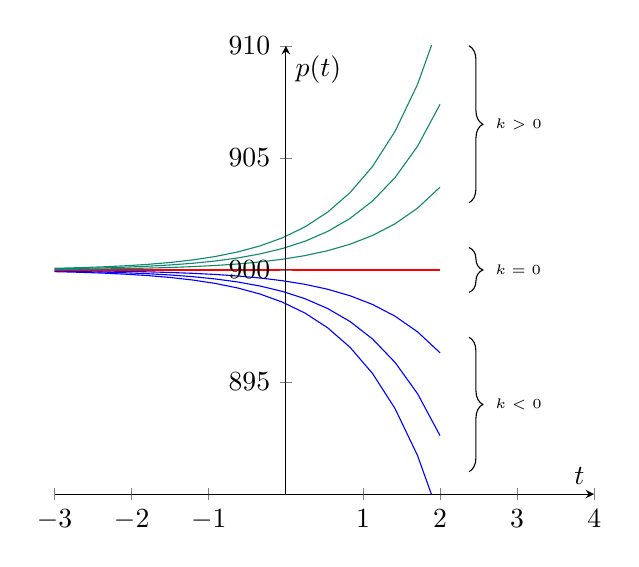
\begin{tikzpicture}
	\begin{axis}[
	ymin = 890, ymax = 910,
	xmin = -3, xmax = 4,
	axis lines=center,
	axis on top=true,
	domain=-5:2,
	xlabel={$t$},
    ylabel={$p(t)$},]
    
    \addplot[mark=none, draw=blue, thin]{900 + -3*exp{x/2}};
    \addplot[mark=none, draw=blue, thin]{900 + -2*exp{x/2}};
    \addplot[mark=none, draw=blue, thin]{900 + -1*exp{x/2}};
    \addplot[mark=none, draw=red, thin]{900 + 0*exp{x/2}};
    \addplot[mark=none, draw=PineGreen, thin]{900 + 1*exp{x/2}};
    \addplot[mark=none, draw=PineGreen, thin]{900 + 2*exp{x/2}};
    \addplot[mark=none, draw=PineGreen, thin]{900 + 3*exp{x/2}};
	\draw [decorate, decoration={brace,amplitude=5pt,raise=1pt,mirror}] (2.34,903) -- (2.34,910) node [midway, xshift=-1mm, auto, swap, outer sep=10pt,font=\tiny]{$k > 0$};
	\draw [decorate, decoration={brace,amplitude=5pt,raise=1pt,mirror}] (2.34,899) -- (2.34,901) node [midway, xshift=-1mm, auto, swap, outer sep=10pt,font=\tiny]{$k = 0$};
	\draw [decorate, decoration={brace,amplitude=5pt,raise=1pt,mirror}] (2.34,891) -- (2.34,897) node [midway, xshift=-1mm, auto, swap, outer sep=10pt,font=\tiny]{$k < 0$};
	\end{axis}

\end{tikzpicture}
\end{center}
\begin{definition-N}
	Here the singular solution $p(t) = 900,$ $\forall t$ is called an \underline{equilibrium solution} (or a \underline{steady-state solution.}) Equilibrium solutions will be important to us in the future.
\end{definition-N}
\redhline\\
Notice in both \circled{a} and \circled{b} above
\begin{center}
	$\dfrac{dy}{dx}$ = something involving $x, y$ \quad \quad $\dfrac{dp}{dt}$ = something involving $p, t$
\end{center}
This is useful since solutions "live" in the x,y-plane or the t,p-plane, only solution curve will hhave its tangent line at $(x, y)$ with slope given by simply evaluating the RHS at that point.\\

\textbf{Example:} for $y' = x-e^{\frac{x}{2}}$, choose $(x_0, y_0) = (2,1)$\\
Then $\dfrac{dy}{dx} \bigg|_{x=2, y=1} = 2-e^{2/2} \approx -0.718$\\
\newline
The solution curve passing through $(2,1)$ will have a slope -0.718 there.\\
Without solving thhe ODE, we can take a grid of points in the xy-plane and evaluate these little slope lines. The result is called a \underline{slope field}. 

\begin{center}
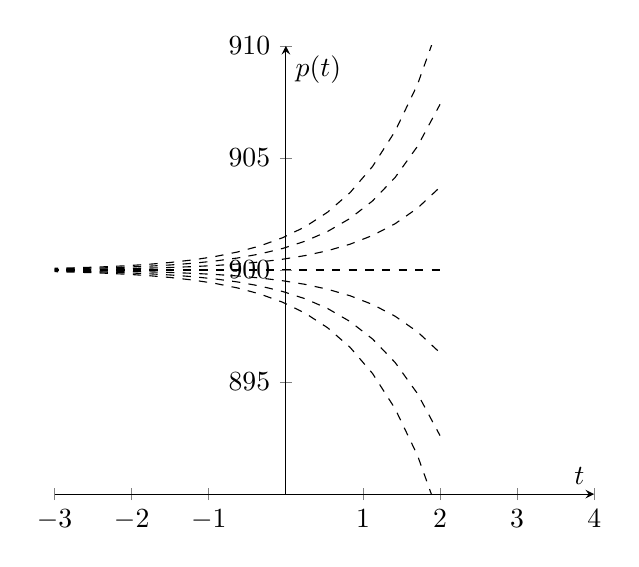
\begin{tikzpicture}
	\begin{axis}[
	ymin = 890, ymax = 910,
	xmin = -3, xmax = 4,
	axis lines=center,
	axis on top=true,
	domain=-5:2,
	xlabel={$t$},
    ylabel={$p(t)$},]
    
    \addplot[mark=none, draw=black, dashed]{900 + -3*exp{x/2}};
    \addplot[mark=none, draw=black, dashed]{900 + -2*exp{x/2}};
    \addplot[mark=none, draw=black, dashed]{900 + -1*exp{x/2}};
    \addplot[mark=none, draw=black, dashed]{900 + 0*exp{x/2}};
    \addplot[mark=none, draw=black, dashed]{900 + 1*exp{x/2}};
    \addplot[mark=none, draw=black, dashed]{900 + 2*exp{x/2}};
    \addplot[mark=none, draw=black, dashed]{900 + 3*exp{x/2}};

	\end{axis}

\end{tikzpicture}
\end{center}
